% Experiments

This section presents the experiments and results aimed at evaluating our proposed graph generative model. First we run a grid-search on the hyperparameter space to find the optimal configuration of the RGVAE. We use the ELBO and MRR as evaluation metric. The best configurations are used to perform link prediction. Here we compare the model performance with vs. without convolutions. We use the VDistMult as control model for link prediction. Finally we run two proof-of-concept experiments. The first generating triples and filter on a entity class constraining relation, thus we get an insight of how much percent of the generated triples are valid. Secondly we analyze the results of a RGVAE trained on subgraphs with $n=10$. For the experiments we use two multi-relational KG datasets.

% We covered link and node prediction and compared those to SOTA scores. Further we ran experiments on investigating the coherence of the reproduced graph structure. Lastly we measured the adherence of our model to the KG's underlying syntax.


\subsection{Data}
\label{ssec5:data}
For this sake of comparison with state of the art results, we chose the two most popular dataset used in this field of KG link prediction, FB15k237 and WN18rr.

% Training models on each dataset for 333 epochs, without early stopping.

\textbf{FB15K-237} is a successor of the FB15K dataset, first introduced by \cite{bordes_translating_2013}, which suffered of major test leakage, meaning that triples from test set could be inferred by inverting triples from the train set. In FB15K-237, introduced in \cite{toutanova_representing_2015} these triples where removed.
The data was scraped from Freebase, while only the most frequent entities and relations were considered. The huge open-world KG Freebase \cite{bollacker_freebase_2008}, which before its discontinuation had around $1.2$ billion triples and $80$ million entities, was structured by assigning types and classes to entities and type constrains to relations. Thus, a triple can only be formed if the relation constrain matches the entity's type. Freebase was free for everyone to access and expand. This led to inconsistencies,duplicates and highly inconsistent notation, which might have been the reason for its discontinuation. Data dumps of the latest version are still available.




% textwidth for figures:
% \printinunitsof{in}\prntlen{\textwidth}

% linewidth for figures:
% \printinunitsof{in}\prntlen{\linewidth}

\textbf{WN18RR}, a dataset of synonyms and hypernyms, is a successor of yet another dataset WN18 introduced by \cite{bordes_translating_2013}. Similar to the the above the original dataset suffered from test leakage, thus, an updated version without reciprocal triples was introduced by \cite{dettmers_convolutional_2018}. This dataset is characterized by its few relations and large corpus of entities. In contrary to FB15K-237, its triples are difficult to be judged on view and the underlying semantics are entity specific, meaning not relying on types and classes.



\begin{table}[H]
  \centering
      \begin{tabular}{|l|l|l|l|}
      \hline
      \rowcolor[HTML]{EFEFEF}
      \multicolumn{1}{|c}{\textsc{Dataset}} & \multicolumn{1}{c}{\textsc{Entities}} & \multicolumn{1}{c}{\textsc{Relations}} & \multicolumn{1}{c|}{\textsc{Triples}}\\\hline
      FB15K-237     & \multicolumn{1}{c|}{$14,951$} & \multicolumn{1}{c|}{$237$} & \multicolumn{1}{c|}{$310,116$}\\
      WN18RR   & \multicolumn{1}{c|}{$40,943$} & \multicolumn{1}{c|}{$11$} & \multicolumn{1}{c|}{$93,003$} \\
      \hline
      \end{tabular}
      \caption{Statistics of the FB15k-237 and WN18RR datasets.}
      \label{tab5:data}
  \end{table}


\subsection{Hyperparameter Tuning}

In this section we run a grid search for the three hyperparameter $\beta$, $d_z$ and $d_h$ for a set of contrastive values. To reduce the computational expenses we train each model for $60$ epochs and  evaluate link prediction on a subset of $50$ triples.

Empirically we set the learning rate to $3e-5$ and the maximum batchsize fitting on the GPU memory. For $d_h$ we did not see any significant changes for higher values, thus we choose a lower number to reduce the total model parameters. The remaining hyperparameter did influence and the optimal setting vary for each dataset, table \ref{tab:RGVAEhyp} shows the results of our hyperparameter tuning.

% lr empirically and batchszize fixed.

% beta
For the hyperparameter tuning of $\beta \in [0,1,10,100]$ we chose significant values. With $\beta = 0$ we do not constrain our model on the Gaussian prior, thus the latent distribution can take the form of any distribution. This reduces the influence of the variational module and the model becomes closer to an autoencoder. For $\beta = 1$ we get our base model, and for $\beta \in [10,100]$ the $\beta-$VAE version.


\begin{figure}[H]
    \centering
    \begin{subfigure}{.5\textwidth}
      \centering
      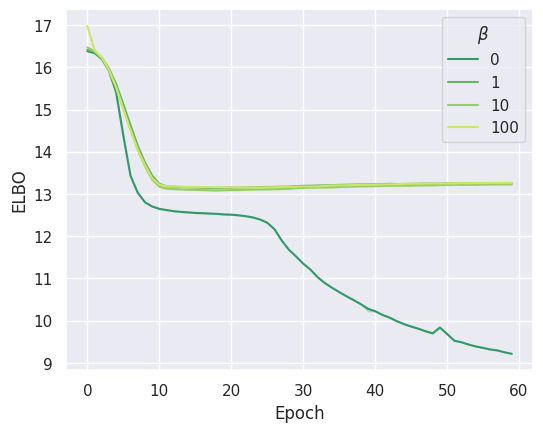
\includegraphics[width=.9\linewidth]{graphs/plots/beta_loss_fb.png}
      \caption{FB15K-237}
      \label{fig5:betafb}
    \end{subfigure}%
    \begin{subfigure}{.5\textwidth}
      \centering
      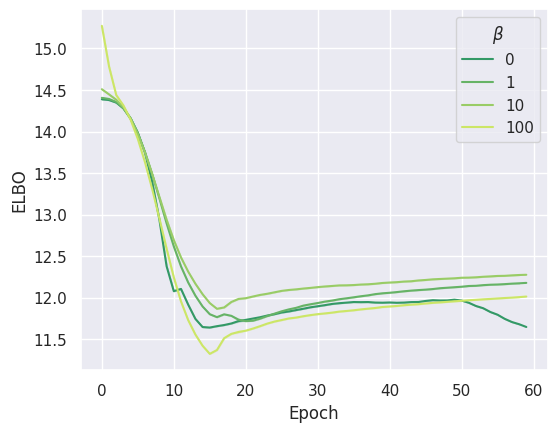
\includegraphics[width=.9\linewidth]{graphs/plots/beta_loss_wn.png}
      \caption{WN18RR}
      \label{fig5:betawn}
    \end{subfigure}
    \caption{Validation loss for RGVAE with $\beta \in [0,1,10,100]$ trained on each dataset.}
    \label{fig5:beta}
\end{figure}


Figure \ref{fig5:beta} shows the validation ELBO for the different $\beta$ values and for both datasets. We notice two interesting outcomes.  

\begin{itemize}
    \item For $\beta = 0$ converges further than the rest.
    \item The remaining values behave quase identical with $\beta = 100$ performing slightly better. 
\end{itemize}

Since setting $\beta = 0$ would undermine our hypothesis of evaluating variational model, we chose $\beta = 100$ as default for the following experiments. This also compares with the $\beta$ values proposed by Higgins in \cite{higgins_beta-vae_2016} to achieve a factorization of the latent space.

Especially on the FB15k-237 dataset the $\beta = 0$ configuration converges to a much lower ELBO. Thus, we have the trained models perform link-prediction on a $1\%$ subset of the validation set. Figure \ref{fig5:betafbmrr} indicates an inverse correlation between the ELBO and the MRR score. 

\begin{figure}[H]
    \centering
      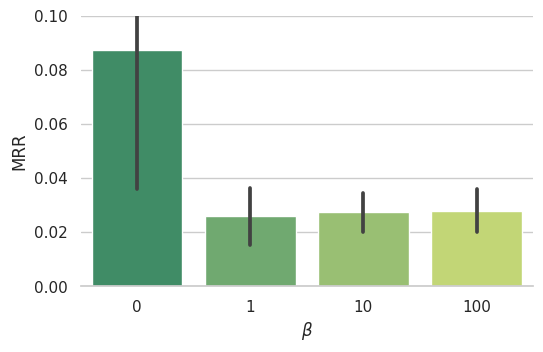
\includegraphics[width=.45\textwidth]{graphs/plots/beta_mrr_fb.png}
      \caption{MRR scores for different $\beta$ values on the dataset FB15k-237.}
      \label{fig5:betafbmrr}
\end{figure}

Barplot IN APPENDIX  

% d_z
Experiments on the impact of $d_z$ on the ELBO show little improvement for $10<d_z<100$ and from $100<d_z<1000$ insignificant to no improvement. Thus, we chose $d_z=100$ as default for our experiments.


% d_h did not influcence
Lastly, we evaluate the models hidden dimensions $d_h$ and its influence on the ELBO and the (subset)MRR. We compare between $d_h\in [256, 512, 1024, 2048]$, while the lowest configuration performs slightly worse on the ELBO, there is no significant difference between the remaining three configurations. Considering the models parameter count we chose the $d_h=512$ as default.


\subsection{Link Prediction}


 We now get to the main experiment of this thesis. The results of this experiment will show if the RGVAE architecture is suitable for link prediction and in first place, if it is able to grasp the underlying KG semantics at least significantly better than random by differentiating between real and corrupted triples. First we evaluate the performance of the RGVAE on this experiment, comparing both encoder versions. Then we investigate the influence of the variational inference by comparing the variational and original versions of DistMult on link prediction.
 
 \subsubsection{RGVAE}

 At this point we bring in the convolutional variation of our model, which we will denote as RGCVAE. The experiments reveal if the convolutional architecture holds an advantage compared to the simple MLP baseline. Further a randomly initiated and untrained RGVAE is used as control model.
 
 Due to its sparse graph computation, the RGVAE takes about 7 days to evaluate link prediction on the full test set and even 3 days when prediction tasks run parallel on a node of $4$ Nvidia Titan RX 25GB GPUs. Since the exemplary link prediction during experimenting with different hyperparameter already gave us an idea of the mediocre performance of our model, we chose to spare computation time and power by running link prediction on a randomly drawn one-third of the complete test set. Each run is repeated three times using a different random seed.

The results are visualized in figure \ref{fig5:lp_final}. We chose a visualization over a table, to emphasize our observations, and for the mentioned limitation of the test set, which makes these results not suitable for academically valid comparisons. Note that the figures are scales and to a range $[0,10]$ while all metrics have a maximum of $1$.

Comparing a MRR of $0.08$ to the DistMult score or $0.4$ our model does not perform competitively on link prediction tasks.

% Better than random?? I hope so.

Graph convolutions do not yield an advantage over the basemodel. In fact, the RGVAE with convolutions even scores slightly worse. 

%  FOR Conclusion: this might be because of the implementation of stacking the matrices.
The model scores about three times better on the FB15k-237 dataset than on WN18RR. FB15k-237 is a richer dataset with more triples and and a more balanced ratio of entities to relations. WN18RR operates on only 18 relations, what makes the relation most crucial when completing a triple. The architecture of the RGVAE puts twice the emphasis entities, described by the adjacency and the node feature matrices, while the relation is only represented by the overly sparse edge attribute matrix. Thus, we could conclude that our model learns to predict based on the hidden types and topics of the entities. All possible conclusions for this are discussed in \ref{sec:discus}. Relevant for this section is solely, that we chose the FB15k-237 dataset to investigate further, how well the RGVAE's grasps the underlying entity types and triple topics.   

%  REASON: fb has more relations, is a more complete KG. wn only 12 relations and more entities. Model emphasizes entities (adj and node features), relations may be less relevant, wn is more about the relation (same/ not the same). This indicates that our model grasps the hidden types and topics of the FB entities.


 \begin{figure}[H]
  \centering
  \begin{subfigure}{.5\textwidth}
    \left
    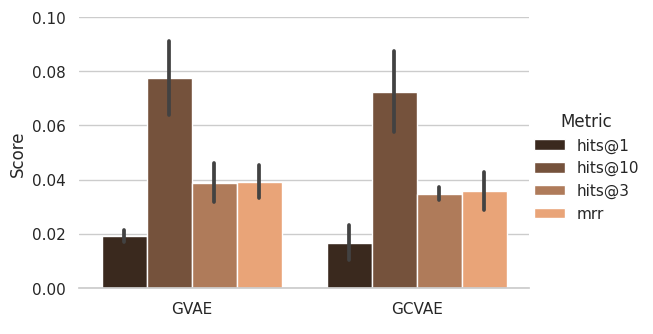
\includegraphics[height=.5\textwidth, keepaspectratio]{graphs/plots/lp_fb.png}
    \caption{FB15K-237}
    \label{fig5:lpfb}
  \end{subfigure}%
  \begin{subfigure}{.5\textwidth}
    \right
    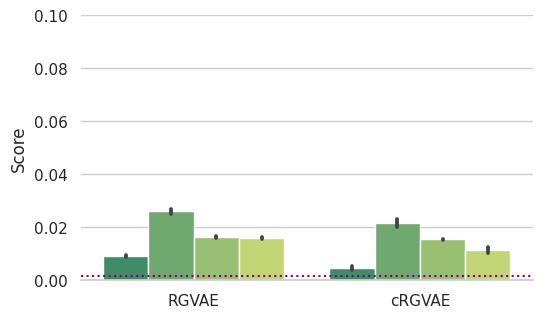
\includegraphics[height=.5\textwidth]{graphs/plots/lp_wn_wol.png}
    \caption{WN18RR}
    \label{fig5:lpwn}
  \end{subfigure}
  \caption{Link prediction results in MRR, Hits@1, Hits@3 and Hits@10 for RGVAE and RGCVAE trained on the full trainset of each dataset.}
  \label{fig5:lp_final}
\end{figure}

% TODO add random!!!

% Compare with vs without convolution 
% We use negative elbo as scoring function. Since elbo is aimed to be reduced and LP scores are higher better.

% We try with and without permutation

% We try the model as encoder only NO

% We use 1/3 of the test set only, randomly drawn. Run 3 times?
% Final models only 60 epochs


\subsubsection{Impact of Variational Inference and Gaussian prior}

In order to explain the poor performance of the RGVAE on the task of link prediction, we investigate the impact of the variational inference. Since the RGVAE with relaxed latent space, meaning less variance, indicated higher scores than the version with Gaussian prior, we examine the two variants by means of embedding models. The original DistMult model with optimized parameter serves as control model, while we compare it to the VDistmult, described in section \ref{ssec4:vdistm}, learning the full ELBO versus learning only on the reconstruction loss. By not including the regularization term in the loss the model is no longer bound to the Gaussian prior, which results in a relaxation of the latent space.

We train the three models for $300$ epochs solely on the FB15k-237 dataset and evaluate MRR, Hits@$1$, Hits@$3$ and Hits@$10$. Table \ref{tab5:VarDistM} shows the mean scores with $\mu \pm \sigma$ of three runs per model. Note that the exponent on $\sigma$ holds for the whole term. We can clearly see that both variational versions of the DistMult perform significantly worse than the original model. Learning on the full elbo or only the reconstruction loss does not seem to influence the scores in this setting. This indicates, that the models performance on link prediction suffers from using variational inference.

In the last row we show the results of the RGVAE with relaxed latent space. This model was trained with $\beta=0$ thus not constraining the latent space on a Gaussian prior. The model outperforms the versions with hyperparameter choice $\beta>0$ and scores the closest to the DistMult model. The impact of $\beta$ shows in the regularization, which we tracked separately. The maximum values of$D_{K L}$ during the experiment are 

\begin{equation}
  \begin{align}
    D_{reg} &= \beta D_{K L}\left(q_{\phi}\left(\mathbf{z} \mid G\right) \| p_{\theta}(\mathbf{z})\right) \\
    \max_{\beta = 0} D_{K L} &= 3506 \\
    \max_{\beta = 100} D_{K L} &= 0.0154
  \end{align}
  \label{eq5:KLdifferentBeta}
\end{equation}


While the results of the relaxed RGVAE might seem promising, Distmult is a much simpler and faster link predictor, thus we do not see a justification to keep researching on the RGVAE for this task. Note that due to the high computation cost of the RGVAE we only run the experiment once on the full dataset.

% TODO: Answer question:Link prediction with control model:

% Trained for 300 epochs

% We see that the variational part messes everything up.

% Table:
% MRR + Hits@all + Loss

\begin{table}[H]
  \centering
      \begin{tabular}{|l|l|l|l|l|}
      \hline
      \rowcolor[HTML]{EFEFEF}
      \multicolumn{1}{|c}{\textsc{Model}} & \multicolumn{1}{c}{\textsc{MRR}} & \multicolumn{1}{c}{\textsc{Hits@$1$}} & \multicolumn{1}{c}{\textsc{Hits@$3$}} & \multicolumn{1}{c|}{\textsc{Hits@$3$}} \\\hline
      DistMult     & \multicolumn{1}{c|}{$0.2854\pm 0.0025$} & \multicolumn{1}{c|}{$0.2\pm 0.001$} & \multicolumn{1}{c|}{$0.3149\pm 0.0038$} & \multicolumn{1}{c|}{$0.4512\pm 0.0053$}  \\
      VDistMult   & \multicolumn{1}{c|}{$0.517\pm 0.0197e^{-3}$} & \multicolumn{1}{c|}{$0.2442\pm 0.1994e^{-4}$} & \multicolumn{1}{c|}{$0.8145 \pm 0.3049e^{-4}$} & \multicolumn{1}{c|}{$0.399\pm 0.0576e^{-3}$} \\
      VDistMult w/ ELBO   & \multicolumn{1}{c|}{$0.6397\pm 0.0357e^{-3}$} & \multicolumn{1}{c|}{$0.57\pm 0.3046e^{-4}$} & \multicolumn{1}{c|}{$0.1547\pm 0.1023e^{-3}$} & \multicolumn{1}{c|}{$0.6351\pm 0.1992e^{-4}$} \\
      RGVAE w/o ELBO   & \multicolumn{1}{c|}{$0.1412$} & \multicolumn{1}{c|}{$0.0981$} & \multicolumn{1}{c|}{$0.1494$} & \multicolumn{1}{c|}{$0.2275$} \\
      \hline
      \end{tabular}
      \caption{Link prediction scores of DistMult and RGVAE versions on the FB15k-237 dataset.}
      \label{tab5:VarDistM}
  \end{table}


\subsection{Impact of permutation}
% Check if adj matrix adheres to edge attribute matrix.

Furthermore we examine the influence of the permutation invariant loss function described in \ref{ssec4:loss}. During training and subset link prediction no significant difference was observed between the RGVAE with versus without matching target and prediction graph. Yet, two observations draw our attention, namely:

\begin{itemize}
  \item The amount of nodes permuted per batch converges during training from $100$\% to exactly $60$%.
  \item The RGVAE with permutation invariant loss function learns to predict many variations of adjacency matrix while the standard model predicts similar to the target.
\end{itemize}

The first point indicates that the model learns a set of adjacency matrices, which can be permuted to match the target while optimizations the loss. Note that the generated matrix representation of the triples either has only one edge on the right upper index $A_{0,n}$ or, in the rare case of self-loops in $A_{0,0}$. The number of nodes per graph for these observations is set to $n=2$. Curiosity remains why the model converges to steadily permute $\frac{3}{5}$ of the prediction.
Secondly, we see that even when converged, the model predicts variations od the adjacency matrix very different to the target. The most common is a single edge on $A_{n,0}$ and on $A_{n,n}$. Less common and with lack of explanation are the predictions of an empty, or multi edge adjacency matrix. In contrast to this and as expected, the RGVAE with the standard loss function learns to solely predict edges on $A_{0.0}$. 
Finally we will analyze the impact of permutation invariance on the experiment of syntax coherence in section \ref{ssec5:syntax}.


% Permutation starts at $100\%$ at the beginning of training and converges to $60\%$.

% Model without predicts adj node always in the upper right just as the target. Model with predicts much more variations of adjacency.

% Graph of permutation during training.
% loss with vs without 

\begin{figure}
  \caption{(a) Validation loss RGVAE with vs. w/o permutation invariant loss function. (b) Percentage of permuted nodes during training.}
  \label{fig5:permInv}
\end{figure}

\subsection{Interpolate Latent Space}

Inspired by the popular results of Higgins, who featurized each latent dimension on a facial features of the FACES dataset \cite{ebner_facesdatabase_2010}. The VAE generates faces controlling feature such as age, gender and emotions by manipulating single latent dimensions \cite{higgins_beta-vae_2016}.  We run this experiment with the RGVAE on the FB15k-237 dataset, using two different interpolation methods. The latent dimension for this experiment is set to $d_{z}=10$ in order to analyze each dimension separately and the interpolation is linear with a step count of $10$.

The first experiment is linear interpolating between two triples. Therefor two valid triples from the train set are encoded into their latent representation. We chose the two semantically related triples triples to analyze if the linear movement in latent space correlates with an obvious semantic feature. 

\begin{center}
  \texttt{[['/m/02mjmr Barack Obama'], ['/people/person/place\_of\_birth'], ['/m/02hrh0\_	Honolulu']]}
  \texttt{[['/m/058w5 Michelangelo'], ['/people/deceased\_person/place\_of\_death'], ['/m/06c62	Rome']]}
\end{center}


% TODO present the results and link to appendix

\begin{table}[H]
  \centering
  \begin{tabular}{|c|}
  \hline
  \rowcolor[HTML]{EFEFEF} 
  \textsc{RGVAE permutation}\\ \hline
  \texttt{[[France] [/base/petbreeds/city\_with\_dogs/top\_breeds] [Imperial Japanese Army]]}\\
  \texttt{[[Cree Summer] [/tv/tv\_program/program\_creator] [David Chase]]}\\
  \texttt{[[Guitar] [/business/business\_operation/assets] [Paramount Vantage]]}\\
  \texttt{[[Democratic Party] [/music/genre/artists] [Howard Hawks]]}\\
  \texttt{[[Roy Haynes] [/people/person/spouse\_s] [The Portrait of a Lady]]}\\
  \texttt{[[Cleveland Browns] [/film/actor/dubbing\_performances] [David Milch]]}\\
  \texttt{[[Jay-Z] [/film/special\_film\_performance\_type/film\_performance\_type] [Ashley Tisdale]]}\\
  \texttt{[[Phoenix Suns] [/film/film/dubbing\_performances] [Lynn]]}\\
  \texttt{[[James E. Sullivan Award] [/organization/organization/child] [Giant Records]]}\\
  \texttt{[[Boston United F.C.] [/soccer/football\_player/current\_team] [Kensal Green Cemetery]]}\\  
  \hline
  \end{tabular}
\caption{Latent space interpolation between two triples in $10$ steps.}
\label{tab5:ipbtw2}
\end{table}
% Obama triple is not reproduced, not even close.

For the second experiment, we interpolate each latent dimension isolated in a $95\%$ confidence interval of the Standard Gaussian distribution. Starting with the encoded representation of the Obama triple, we incrementally add $z_{i} += -1.96 + j \times s$ with $s = \frac{1.96 * 2}{n_s-1}$ for the number of steps $n_s = 10$. Due to the size of the tables representing the interpolations and the low value they add to the presentation of this work, the result of this experiments can be found in the appendix.


% Further we go ahead and test what happens if we modify one latent dimension at a time with $d_z = 10$ of a triple. TABLE: (s,r,o), x axis dims, y axis steps. $95\%$ Gaussian confidence 

% Can the model assign logical features to latent dimensions?


\subsection{Syntax coherence}
\label{ssec5:syntax}

On closed-world schema-based KGs the approach for testing the validity of a new triple is to add it to the existing KG and run a onthology reasoner on it. A inconsistency in the KG will appear as \texttt{null}-Class, but only if an axiom is violated. This approach works only for fully constrained KGs and is not scalable, since the reasoner recursively checks evey triple for every axiom. Thus, we present an alternative and improvised way to estimate the validity of generated triples.

The FB15k-237 is a subset from the FreeBase KG \cite{bollacker_freebase_2008}, thus, even thought they are not part of the dataset, - entities have type properties in their original Freebase representation. 
Querying the last official Freebase dump, we get the types for each entity in the FB15k-237 dataset, With exception of $8$ entities, which could not be found in the query.

Our approach is to randomly generate triples, from signals randomly drawn from a Standard Gaussian distribution. Then to filter those triples on predicates which contain the type \textit{people}, which is within the top 10 most common Freebase types. We differentiate between base-class types subclass types, both can contain the word \textit{people}. The entity \texttt{['/m/02mjmr Barack Obama']} has between many others the type \texttt{[/people/measured\_person]}. Here the base class is \textit{people} and the subclass \textit{measured\_person}. We could filter directly on subclasses, but we chose to give our model more creative freedom and filter for \textit{people} in the full set of types. Using this choice, the generated triples are scored on logic rather than facts. E.g. any person can hypothetically the a \textit{measured\_person}, understanding this implies semantical reasoning, while differentiating between which person is and is not a \textit{measured\_person} implies contextual knowledge. Thus, we use the base type \textit{people} to validate triples.
Furthermore the relations are inconsistent in their notation, partly not only having a head type constrain. Thus, we check only the head entity for the key type. 

\begin{itemize}
  \item From $14541$ entities, $5283$ contain the keyword people, or $36.332$\%.
  \item From $237$ predicates, $25$ contain the keyword people, or $10.549$\%.
  \item From $310116$ triples, $47354$ contain the a predicate keyword people, or $15.269$\%.
\end{itemize}

Considering these facts, we calculate the marginal probability of guessing a head entity $s$ of type \textit{people}, given a triple which contains the type \textit{people}. Without prior knowledge $p(s_{p})$ and $p(r_{p})$ are conditionally independent. The probability is calculated as:

\begin{equation}
  p(s_{p} \mid r_{p}) &= p(s_{p}) = 0.3633
  \label{eq5:randomValid}
\end{equation}

For this experiment we generate triples until $10e^5$ contain the key type. Those filtered triples are validated on the type of the head entity and compared to the full dataset for novelty. Here we again compare the performance between the RGVAE with the two different encoder architectures. Furthermore the models are trained both with regular and permutation invariant loss function. Lastly, the experiments are repeated for sampling the latent signal from $\mathcal{N}(0,1)$ and for sampling from $\mathcal{N}(0,2)$.  We average the accuracy of three runs of generating a valid triple and of this triple being unseen in the dataset. The results for valid triples are shown in figure \ref{fig5:syntax}. The dotted horizontal line indicates the random probability of generating a valid triple, calculated in equation \ref{eq5:randomValid} and $\sigma^2_1$ and $\sigma^2_2$ denote the variance for the different latent space distributions. 



\begin{figure}[H]
  \centering
  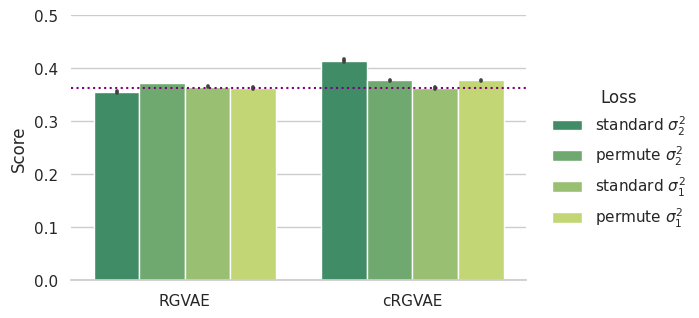
\includegraphics[height=.25\textwidth, keepaspectratio]{graphs/plots/kg_all.png}
  \caption{Accuracy of generating valid triples.}
  \label{fig5:syntax}
\end{figure}

To our disappointment the model does not perform significantly better than random. Neither the choice loss function nor the doubled variance show a correlation with the accuracy. The only configuration standing out is the RGVAE with convolutional encoder, standard loss function and $\sigma^2=2$, scoring $4$\% higher than random. From all valid generated triples $100\pm 0.001$\% are new and unseen in the dataset. Coming back to \texttt{['/m/02mjmr Barack Obama']}, we filter the unseen triples fo the first three appearances of this entity. These are displayed in table \ref{tab5:genTriples} for every variation of the RGVAE and in the same order as in figure \ref{fig5:syntax} 



\begin{table}[H]
  \begin{tabular}{|c|}
  \hline
  \rowcolor[HTML]{EFEFEF} 
  \textsc{RGVAE standard} $\sigma_2^2$\\ \hline
  \texttt{[[Barack Obama]	[/people/person/places\_lived./people/place\_lived/location]	[Casablanca]]}\\
  \texttt{[[Barack Obama]	[/people/person/place\_of\_birth]	[Sarah Silverman]]}\\
  \texttt{[[Barack Obama]	[/people/person/place\_of\_birth]	[The League of Extraordinary Gentlemen]]}\\ \hline
  \rowcolor[HTML]{EFEFEF} 
  \textsc{RGVAE permuted} $\sigma_2^2$\\ \hline
  \texttt{[[Barack Obama]	[/people/ethnicity/geographic\_distribution]	[End of Watch]]}\\
  \texttt{[[Barack Obama]	[/people/profession/specialization\_of]	[Montgomery County]]}\\
  \texttt{[[Barack Obama]	[/people/cause\_of\_death/people]	[WWE Superstars]]}\\ \hline
  \rowcolor[HTML]{EFEFEF} 
  \textsc{RGVAE standard} $\sigma_1^2$\\ \hline
  \texttt{[[Barack Obama]	[/people/person/place\_of\_birth]	[Academy Award for Best Sound Editing]]}\\
  \texttt{[[Barack Obama]	[/people/person/places\_lived./people/place\_lived/location]	[Stan Lee]]}\\
  \texttt{[[Barack Obama]	[/people/person/place\_of\_birth]	[Multiple sclerosis]]}\\ \hline
  \rowcolor[HTML]{EFEFEF} 
  \textsc{RGVAE permuted} $\sigma_1^2$\\ \hline
  \texttt{[[James Brolin]	[/people/person/places\_lived./people/place\_lived/location]	[Barack Obama]]}\\
  \texttt{[[Barack Obama]	[/people/person/spouse\_s./people/marriage/location]	[D.C. United]]}\\
  \texttt{[[Jim Sheridan]	[/people/person/religion]	[Barack Obama]]}\\ \hline
  \rowcolor[HTML]{EFEFEF} 
  \textsc{cRGVAE standard} $\sigma_2^2$\\ \hline
  \texttt{}\\
  \texttt{None}\\
  \texttt{}\\ \hline
  \rowcolor[HTML]{EFEFEF} 
  \textsc{cRGVAE permuted} $\sigma_2^2$\\ \hline
  \texttt{[[Pinto Colvig]	[/people/deceased\_person/place\_of\_burial]	[Barack Obama]]}\\
  \texttt{[[Helena Bonham Carter]	[/people/person/gender]	[Barack Obama]]}\\
  \texttt{[[John Buscema]	[/people/person/spouse\_s./people/marriage/spouse]	[Barack Obama]]}\\ \hline
  \rowcolor[HTML]{EFEFEF} 
  \textsc{cRGVAE standard} $\sigma_1^2$\\ \hline
  \texttt{[[Suhasini Ratnam]	[/people/person/sibling\_s./people/sibling\_relationship]	[Barack Obama]]}\\
  \texttt{[[Barack Obama]	[/people/person/gender]	[Deva]]}\\
  \texttt{[[Barack Obama]	[/people/person/sibling\_s./people/sibling\_relationship]	[Niagara Falls]]}\\ \hline
  \rowcolor[HTML]{EFEFEF} 
  \textsc{cRGVAE permuted} $\sigma_1^2$\\ \hline
  \texttt{[[Jonathan Rhys Meyers]	[/people/person/nationality]	[Barack Obama]]}\\
  \texttt{[[Barack Obama]	[/people/person/sibling\_s./people/sibling\_relationship]	[Motherwell F.C.]]}\\
  \texttt{[[Pinto Colvig]	[/people/deceased\_person/place\_of\_burial]	[Barack Obama]]}\\ \hline
  \end{tabular}
\caption{Generated and unseen knowledge.}
\label{tab5:genTriples}
\end{table}


The generated triples confirm the accuracy results. With exception of the triple 
\begin{center}
  \texttt{[[Barack Obama]	[/people/person/places\_lived./people/place\_lived/location]	[Casablanca]]} 
\end{center}

all remaining triples violate common sense logic. The RGVAE does not differentiate between the types gender, location, movie, person or medicine. It even goes so far to state that Obama was born in \texttt{[Multiple sclerosis]}. While this might sound funny it also clearly indicates, that our model did not learn the underlying semantics of this real world KG.

While investigating the model and the generated triple set, we notice two outcomes. Neither the augmentation of the variance nor the enabling of the permutation invariance has an impact on either of the model with two encoder versions. The regularization loss converges during training to zero, meaning that the model learns a latent representation of the dataset as  nearly perfect Standard Gaussian distribution. Yet, even when sampling latent signal from the exact same distribution, we notice that each model repeatedly predicts combinations of a small subset of entities and relations, e.g. the RGVAE version which did not predict the Obama entity once in a total of $111583$ valid triples. This also aligns with the interpolation results, where we observed a static relation for the full gridsearch of the latent space. If we look at the gradient and parameter values $\phi$ and$\theta$ of the MLP encoder and decoder, we see a much higher variance and gradients for $\phi$. The decoder shows higher values and variance for a small subset of neighboring parameter, while the remaining parameters converge to a very similar and low value. This indicates that the encoder learns very well to represent each different triple as Standard Gaussian latent representation. The decoder MLP on the opposite seems to to ignore most of this representation by assigning vanishing values to the connected parameters. Intuitively it seems that the decoder learns to interpret the part of the latent representation corresponding to the adjacency matrix and minimizes as well as stabilizes the loss of the edge and node attribute matrix by uniformly distributing their probability. This leads to the decoder reconstructing edge and node attribute randomly. Further, depending on the values of $\theta$ when the model finishes learning, the decoder will keep predicting the same subset of entities and relation independent of the latent signal $z$. If we look at the flattened representation of our input graph, we see that the part representing the adjacency matrix is way shorter and has a tractable mean of $\frac{1}{4}$ while the mean for the edge and node attribute matrices are $\frac{1}{{4 \times 1345}}$ and $\frac{1}{14951}$. The problem of a our decoder partly ignoring the latent input and potential solutions are discussed further in section \ref{ssec7:collapse}. 


\subsubsection{Delta Correction}
\label{ssec5:delta}


% Explain quick delta implementation 

% Explain new experiments

% show interesting interpolation

% show parameters if different

\begin{figure}[H]
  \centering
    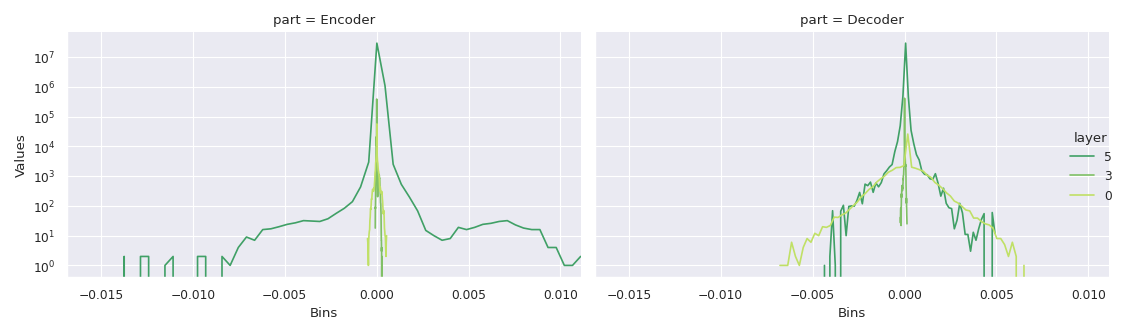
\includegraphics[width=\textwidth]{data/ip/GVAE_p1_delta_encoder.png}
    \caption{MRR scores for different $\beta$ values on the dataset FB15k-237.}
    \label{fig5:deltaParams}
\end{figure}


\begin{figure}[H]
  \centering
    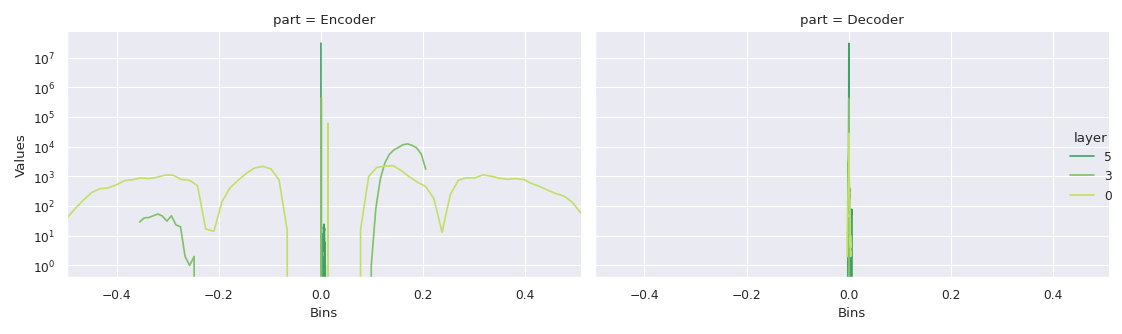
\includegraphics[width=\textwidth]{data/ip/GVAE_p1_encoder.png}
    \caption{MRR scores for different $\beta$ values on the dataset FB15k-237.}
    \label{fig5:normParams}
\end{figure}
